\documentclass[runningheads,svgnames]{llncs}
%
\usepackage[]{graphicx}
\usepackage{amsmath}
\usepackage{hyperref}
\usepackage{cleveref}
% \usepackage{tikz}
% \usepackage{nth}
\usepackage{booktabs}
% \usepackage{array}
\usepackage{orcidlink}
\usepackage{subcaption} % Addition
\usepackage{multirow} % Addition
\usepackage{tabularx} % Addition
\usepackage{siunitx} % Addition
\usepackage{scalerel}
\usepackage[inline,shortlabels]{enumitem}
\usepackage{xspace}


% \usetikzlibrary{shadings,decorations,decorations.pathreplacing}
\renewcommand\UrlFont{\color{blue}\rmfamily}
% FIXME proper hyperref setup

\newcommand{\mcite}[1]{\text{\cite{#1}}}
\newcommand{\mref}[1]{\text{\ref{#1}}}

% \renewcommand{\baselinestretch}{0.97}
\newcommand{\peroocr}{PERO OCR\xspace}


% Comment 
% FIXME : delete before submission :)
\newcommand{\bertrand}[1]{\textcolor{violet}{Bertrand:~#1}}
\newcommand{\nathalie}[1]{\textcolor{purple}{Nathalie:~#1}}
\newcommand{\edwin}[1]{\textcolor{pink}{Edwin:~#1}}
\newcommand{\joseph}[1]{\textcolor{red}{Joseph:~#1}}

% Customize table rendering
\setlength{\tabcolsep}{5pt}
\renewcommand{\arraystretch}{1.4}

\begin{document}
%
\title{A Benchmark of Named Entity Recognition Approaches in Historical Documents\\
Application to 19$^{th}$ Century French Directories%
% FIXME "19$^{th}$-Century" with dash?
% \thanks{%
% This work was supported by the French National Research Agency:
% Project SoDuCo, grant ANR-18-CE38-0013.% ???FIXME need acknowledgments for directory sources???
% }
}
%
\titlerunning{A Benchmark of NER Approaches in Historical Documents}
%
\author{%
N. Abadie\inst{1}\orcidlink{0000-0001-8741-2398} \and
E. Carlinet\inst{2}\orcidlink{0000-0001-5737-5266} \and
J. Chazalon\inst{2}\orcidlink{0000-0002-3757-074X} \and
B. Duménieu\inst{3}\orcidlink{0000-0002-2517-2058}\\
{\footnotesize \emph{all authors contributed equally}}%
}
%
\authorrunning{N. Abadie et al.}
%
\institute{%
% 1
LASTIG, Univ. Gustave Eiffel, IGN-ENSG, F-94160 Saint-Mandé, France\\
\email{nathalie-f.abadie@ign.fr}%\\
% \url{https://www.umr-lastig.fr/nathalie-abadie/}%
\and
% 2
EPITA Research \& Development Laboratory (LRDE), Le Kremlin-Bicêtre, France\\
\email{\{edwin.carlinet,joseph.chazalon\}@lrde.epita.fr}%\\
%\url{https://lrde.epita.fr}
\and
% 3
CRH-EHESS, Paris, France\\
\email{bertrand.dumenieu@ehess.fr}%\\
% \url{http://crh.ehess.fr/index.php?5206}\\
}
%
\maketitle              % typeset the header of the contribution
%
\begin{abstract}
% !TeX root = ../main-paper.tex
Named entity recognition (NER) is a necessary step in many pipelines targeting historical documents.
Indeed, such natural language processing techniques identify which class each text token belongs to,
e.g. ``person name'', ``location'', ``number''.
Introducing a new public dataset built from 19th century French directories,
we first assess how noisy modern, off-the-shelf OCR are.
Then, we compare modern CNN- and Transformer-based NER techniques
which can be reasonably used in the context of historical document analysis.
We measure their requirements in terms of training data,
the effects of OCR noise on their performance,
and show how Transformer-based NER can benefit from unsupervised pre-training 
and supervised fine-tuning on noisy data (\cref{fig.pipeline-overview}).
Results can be reproduced using resources available at \url{https://github.com/soduco/paper-ner-bench-das22}.
% The latest version of is paper can be obtained at \url{https://arxiv.org/abs/xxxx.xxxxx}.
\keywords{Historical documents \and Natural Language Processing \and Named Entity Recognition \and OCR noise \and Annotation cost.}
\end{abstract}

% ---- Sections ----
% !TeX root = ../main-paper.tex
\begin{figure}[!h]
    \centering
    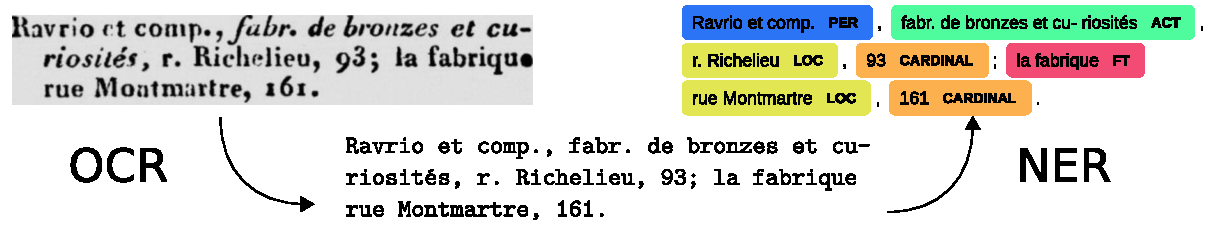
\includegraphics[width=.9\textwidth]{figs/overview-intro.pdf}
    \caption{%
    Overview of the pipeline under study.
    From previously-extracted images of directory entries, 
    we perform OCR and named entity recognition (NER) using different techniques.
    We aim at answering the following questions:
    \emph{How noisy are modern, out-of-the-box OCR systems?}
    \emph{What is the behaviour of NER when OCR is noisy?}
    \emph{Can NER be made more robust to OCR noise?}
    }
    \label{<label>}
\end{figure}
\clearpage% force float flush!

\section{Introduction}

% General context + scope limitation
OCRed texts are generally not sufficient to build a high level semantic view of a collection of historical documents.
A subsequent stage is often needed to extract the pieces of information most likely to be searched for by users, such as named entities: persons, organisations, dates, places, etc.
Indeed, being able to properly tag text tokens unlocks the ability to relate entities and provide colleagues from other fields with databases ready for exploitation.

Being active research topics, OCR and named entity recognition (NER) are still difficult tasks when applied to historical text documents.
OCR approaches used for modern documents are likely to struggle even on printed historical documents due to multiple causes related to text readability (low resolution scans, inconsistent printing rules, artefacts, show-through), document complexity (intricate and versatile page layout, use of ancient fonts \& special glyphs) and the variability inherent to the great diversity of historical sources.
On the other hand, the semantics of entities in NER approaches developed for modern texts may be different from those in ancient texts.

In this article, we focus on a corpus of printed trade directories of Paris from the XIX\textsuperscript{th} century, containing hundreds of pages long lists of people with their activity and address.
They provide fine-grained knowledge to study the social dynamics of the city over time.
As they originate from different publishers, they show a diversity in layout, information organisation and printing quality, which adds to the poor digitising quality to make OCR and NER challenging tasks.

Trade directories have been leveraged in a recent work to identify polluted urban soils \cite{bell2020automated} and locate all gas stations in the city of Providence over the last century.
In an ongoing research project we aim at producing structured spatio-temporal data from the entries in the Paris trade directories to study the transformations of the fraction of XIX\textsuperscript{th} century Parisian society reachable through these sources.
%Because they originate from several publishers, their content is organised following different indexing methods (by name, by activity or by address), is printed in various layouts, and uses different fonts.
Therefor, we investigate several state-of-the-art OCR and NER approaches to assess their usability to process the corpus.

The contributions of this article are the following.
% Contributions
\begin{enumerate*}[(i)]
    \item We review state of the art OCR and NER systems for historical documents (\cref{sec:related-work}).
    \item We introduce a new dataset suitable for OCR and NER evaluation (\cref{sec:dataset}).
    \item We measure the performance of three modern OCR systems on real data (\cref{sec:ocr-xp}).
    \item We evaluate modern NER approaches: their requirements in terms of training data, and the effects of pre-training (\cref{sec:ner-xp1}).
    \item We show that Transformed-based NER can benefit from pre-training and fine-tuning to improve its performance on noisy OCR (\cref{sec:ner-xp2}).
\end{enumerate*}



% !TeX root = ../main-paper.tex
\section{OCR and NER on historical texts}
\label{sec:related-work}

\joseph{Suggestion pour réduire la présentation de l'état de l'art : l'orienter exclusivement vers une justification des systèmes que nous avons retenus pour cet article.}

The directory processing pipeline presented in \cite{bell2020automated} includes an OCR step, done with Tesseract, and a NER step to identify company names and addresses, performed using regular expressions.
This section reviews existing OCR and NER approaches with historical texts and presents some works assessing the effects of OCR quality on the NER performance and the proposed solutions. 

\subsection{Optical Character Recognition on historical texts}

Most of the current state-of-the-art OCR systems, like Tesseract \cite{smith2007overview}, OCRopus \cite{breuel2008ocropus} and PERO OCR \cite{kohut2021ts} are based on a pipeline of convolutional neural networks (CNNs) and long short-term memory networks (LSTM).
Although this kind of model produces good results with modern texts, it faces several challenges with ancient texts, such as the lack of annotated data for learning, or different transcription styles in training data.

\cite{martinek2019hybrid} propose an approach to generate synthetic annotated text for historical OCR training, based on manually collected characters from historical text images.
This work proposes to train an OCR system based on a CNN-LSTM network with synthetic data and then to fine-tune the model with some pages of real historical annotated text.
The results show that this approach gives state-of-the-art results. 

To overcome the limitations due to different transcription styles in training data, PERO OCR adds a Transcription Style Block layer to a classical model based on a CNN and a Recurrent Neural Network components \cite{kohut2021ts}.
This block takes the image of the text and a Transcription Style Identifier as inputs and helps the network decide what kind of transcription style to use as output.

\joseph{Move to implementation details for XP OCR or to pipeline summary}
\begin{itemize}
    \item Tesseract 4.1.1 (newest version: 5, released Nov. 2021)
    \item Pero OCR version from git repo, master branch updated on Sep 15, 2021 % 8b20f29    
    \item other?  % kraken if times allows
\end{itemize}


% PERO refs
% O Kodym, M Hradiš: Page Layout Analysis System for Unconstrained Historic Documents. ICDAR, 2021.
% M Kišš, K Beneš, M Hradiš: AT-ST: Self-Training Adaptation Strategy for OCR in Domains with Limited Transcriptions. ICDAR, 2021.
% J Kohút, M Hradiš: TS-Net: OCR Trained to Switch Between Text Transcription Styles. ICDAR, 2021.


\subsection{Named Entity Recognition}

Many approaches have been designed to recognize named entities, ranging from handcrafted rules to supervised approaches \cite{nadeau2007}.
Rule based approaches look for portions of the text that match patterns like in \cite{bell2020automated,nouvel2011} or dictionary (gazetteers, author lists, etc.) entries like in \cite{mansouri2008,maurel2011}.
Such kind of approaches achieve very good results when applied to a specialized domain corpus and when an exhaustive lexicon are available, but at high system engineering cost \cite{nadeau2007}. 

Supervised approaches include both approaches implementing supervised learning algorithms with careful text feature engineering, and deep learning based approaches which automatically build their own features to classify tokens into named entity categories.
In recent years, the latter have grown dramatically, yielding state-of-the-art performances as shown in the recent survey proposed by \cite{li2020}. This survey concludes that fine-tuning general-purpose contextualized language models with domain-specific data is very likely to give good performance for use cases with domain-specific texts and few training data. This strategy has been adopted by \cite{Labusch2020NamedED} to extract named entities in OCRed historical texts in German, French, and English. However, the NER performance decreased dramatically with OCRed texts is noted, especially for the English texts for which the OCR is of poorer quality. 

\subsection{Improving Named Entity Recognition in historical texts}
\label{subsection:stoa-ner-on-historical-texts}


Several recent studies have focused on the extent to which the quality of the OCR affects the results produced by a NER model.
\cite{van2020assessing} assess the impact of OCR on several NLP downstream tasks, including NER. They worked on a corpus published by a post-OCR correction software company, made of many journal articles with different levels of OCR errors and their respective ground truths.
For each OCRed article, the Word Error Rate (WER) is computed and the English model \textit{en-core-web-lg} provided by Spacy\footnote{\url{https://spacy.io/}} library is used to perform NER on \textit{Person}, \textit{GPE}\footnote{Geopolitical Entity} and \textit{Date}.
The performance of the NER model with respect to OCR quality is eventually assessed by computing the F-measure for each NER class, and each article i.e., each WER value.
\cite{hamdi2020assessing} performed a similar but more extensive evaluation on four different NER models: CoreNLP using Conditional Random Fields and three deep neural models, BLSTM-CNN, BLSTM-CRF, and BLSTM-CNN-CRF.
They tested them on two well-known NER benchmark corpora: CoNLL-02 and CoNLL-03. They applied four different types of OCR noise to each corpus, with two levels of degradation and computed the WER and Character Error Rate (CER) for each degraded version.
Finally, they applied each NER model to the progressively degraded versions of the corpus and computed the resulting F-measure.
Overall, NER F-measure drops from 90\% to 50\% when the WER increase from 8\% to 50\%. However, models based on deep neural networks seem less sensitive to OCR errors.

\cite{huynh2020use} and \cite{marz2021data} have proposed different approaches to reduce the negative impact of OCR errors on NER performance with historical texts.
The former uses a spelling correction tool on several corpora with variable OCR error rates, to assess whether NER performance benefit from spelling corrections or not.
As long as OCR errors remain low (CER<2\% and WER<10\%), the F-measure of NER results remains stable.
It starts to decrease significantly when OCR errors exceed these thresholds.
The latter work focuses on adapting the training data to facilitate the generalization of an off-the-shelf NER model from modern texts to historical texts.
Three different NER models are tested on three historical corpora, in French, English, and Dutch. The best results are produced by a model trained on clean modern data, including embeddings computed with Flair on a historical corpus, and fine-tuned on a noisy historical ground truth.

In conclusion, NER approaches based on deep learning seem to be more suitable for dealing with historical texts as they adapt more easily to OCR errors than rule-based approaches.
Recent work in this area suggests that the impact of OCR quality on NER can be reduced by using different strategies.
On the one hand, if the OCR error rate is kept below a certain threshold, the NER models remain little impacted: it is therefore important to reduce OCR errors as much as possible, but a low error rate may remain acceptable.
On the other hand, reusing a NER model trained on modern data and adapted to historical texts using supervised or unsupervised approaches seems a good strategy. 




\subsection{== À réintégrer depuis ancienne section 4 ==}
We select two deep-learning-based NER models available in packaged software libraries: SpaCy NLP pipelines and CamemBERT.


\subsubsection{spacy}
Spacy is a software library that offers NLP components assembled in modular pipelines specialised by language.
Although BERT is available in the latest version of SpaCy (v3), the pipeline for French does not provide a NER layer at the time of our experiments (jan. 2022).
Hence, we rely on SpaCy's ad hoc pipeline trained on French corpora and capable of named entity recognition.
% deep-sequoia and wikiner-fr, capable of named entity recognition.\textit{fr\_core\_news\_lg}\footnote{https://spacy.io/models/fr} trained two corpora in French: deep-sequoia and wikiner-fr, capable of named entity recognition.
The global architecture of these pipelines have not been yet published but are explained by the developers on their website.
Words are first encoded into local context-aware embeddings using a window-based CNN similar to~\cite{collobert2011}.
The decision layer is an adaptation of the transition-based model presented in~\cite{lample2016}.
As words are processed sequentially, their vectors are concatenated with those of the last known entities to encode the nearby predicted semantics.
The classification layer relies on a finite-state machine whose transition probabilities are learned using a multilayer perceptron.
% \bertrand{Drop the next sentences if we need space}
% In 2018~\cite{won2018} evaluated SpaCy's NER ability to detect place names in five corpora of ancient letters written in English.
% They measured an average F1 score of 0.57.
% The SpaCy developers claim an accuracy of 0.85 for the English NER pipeline \textit{en\_core\_web\_lg} on the OntoNotes 5.0 corpus\footnote{https://spacy.io/usage/facts-figures}.
%For our experiments, the French model \textit{fr\_core\_news\_lg} is fine-tuned using our ground truth corpus.


% Other possibilities:
%1. Traditional ML based:
%    Conditional Random Fields (CRF) - https://pypi.org/project/sklearn-crfsuite/
%    Maximum-entropy Markov model

%2. Neural Networks based:
%    LSTMs, bi-LSTM - https://github.com/flairNLP/flair
%    CNNs (SpaCy uses CNN based architecture)
%    Transformers (Spacy has recently launched it) - %https://spacy.io/universe/project/spacy-transformers


\subsubsection{Transformers / Bert / Hugging face}
Language model based on \textit{Transformers} \cite{vaswani2017attention}, like BERT \cite{devlin2018bert}, have become a new paradigm for NER\cite{li2020}. 
The learned embeddings can be used as distributed representations for input instead of traditional embeddings like Google Word2Vec, and they can be further fine-tuned for NER by adding an additional output layer. 
They can also be pretrained in an unsupervised way on historical texts for domain adaptation.
As the directories are written in French, we chose the language model CamemBERT \cite{martin-etal-2020-camembert}, a Transformer model trained on a French corpus.
\joseph{plutôt tourner ça pour dire qu'il existe des modèles FR / qu'on est limités par la dispo de modèles FR pré-entraînés ?}

\subsection{Pipeline summary}

\Cref{fig.protocol} depicts the evaluation protocol used to assess the OCR and NER systems. 

\begin{figure}[tb]
    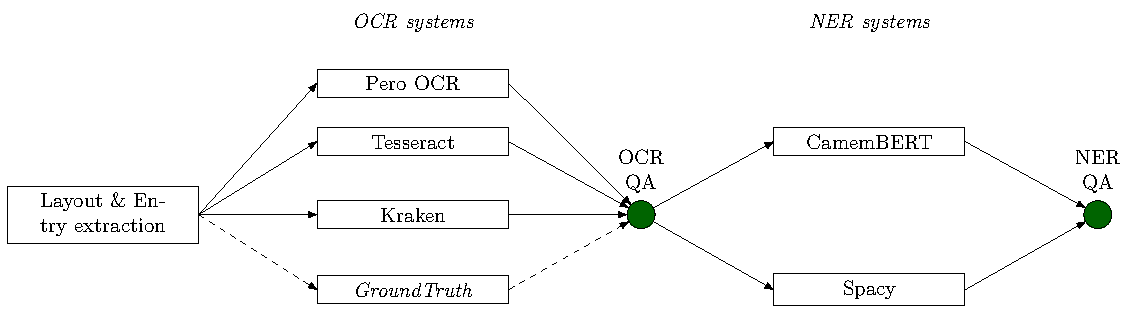
\includegraphics[width=\linewidth]{figs/protocol.pdf}
    \caption{Scheme of the evaluation protocol. \joseph{Missing "Ground truth" for NER stage?}}
    \label{fig.protocol}
    \end{figure}



% !TeX root = ../main-paper.tex
\section{Dataset}

% !TeX root = ../main-paper.tex
\section{OCR benchmark}
\label{sec:ocr-xp}

This section focuses on the evaluation of the performance of the three open-source OCR systems we selected, as described in \cref{sec:pipeline-summary}: Tesseract v4, Kraken and \peroocr.
The dataset used to perform this evaluation is composed of the $8,765$ entries (containing $424,764$ characters) from the dataset we previously introduced.
The single-column, cropped image of entries are used as input of each OCR system after a simple background whitening.
As pages were previously deskewed, text is mostly horizontal except for a few cases.
The expected output is the human transcription of these images provided in the dataset.
Before computing the Character Error Rate (CER) for each entry, each text prediction is normalized with the same basic rules as the ones used to post-process human transcriptions: dashes, quotes, and character code for some glyphs like stars or hands are normalized.
% Regarding the charset of each OCR, Tesseract predicts characters covering a large portion of Latin script, \peroocr generates characters with a similar range, sometimes predicting some Cyrillic characters, and Kraken is constrained by its English model to predict only ASCII characters.


%\subsection{Results and discussion}

\begin{figure}

\subcaptionbox{}[.5\linewidth]{
\begin{tabular}{rlll}
\toprule
 & \peroocr  & Tesseract & Kraken \\    
\midrule
CER & 3.78\% & 6.56\% & 15.72\% \\  
\bottomrule
\end{tabular}
\bigskip

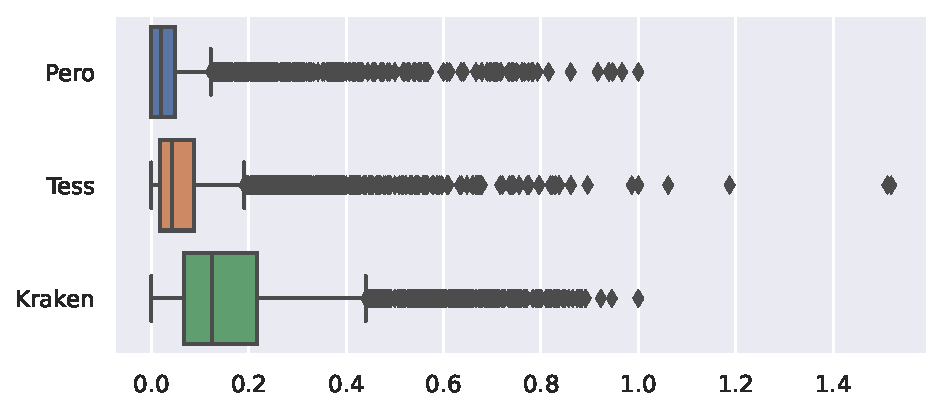
\includegraphics[width=\linewidth]{images/ocr-eval-2.pdf}
\medskip
}
\subcaptionbox{}[.5\linewidth]{
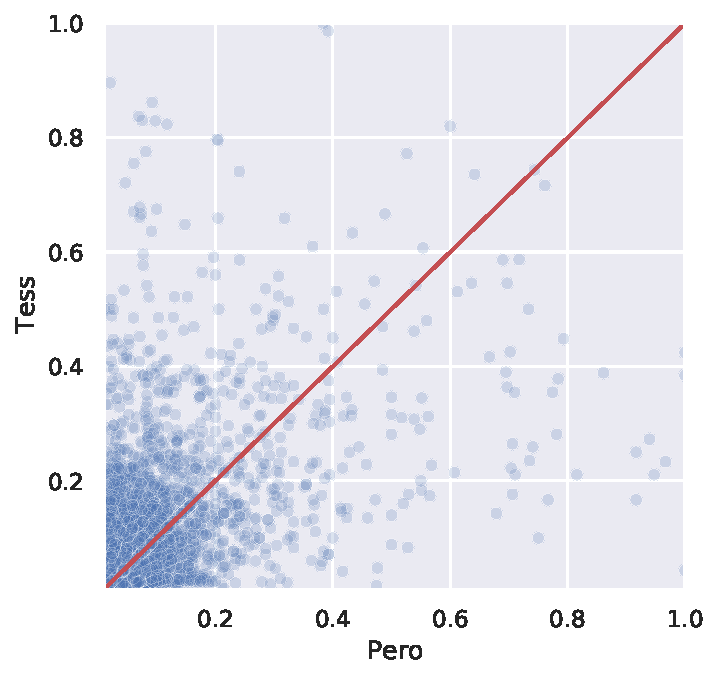
\includegraphics[width=\linewidth]{images/ocr-eval-1.pdf}
}
\caption{CER at entry-level for \peroocr, Kraken and Tesseract. (a) Global CER and distribution of the CER per entry. (b)
joint plot of the per-entry error rate showing that \peroocr and Tesseract do not fail on the same entries.}  
\label{fig.ocr-results}
\end{figure}
%
\Cref{fig.ocr-results} compares the performance of the OCR systems on our dataset. We can see Kraken's performance are
not as good as the two first OCR. This is partially due to the fact that the closest available model is for English text
and so it misses French specific symbols. On the over hand, even when using a French model trained on French 19th
documents, performance does not increase (and relaxing the character matching rules does not help either). Tesseract and
\peroocr are performing better on this dataset ``out-of-the-box''. With no fine-tuning, \peroocr gets the best accuracy
with less than 4\% character errors. Many of them are even due to a bad line detection in case of multi-lines entries
and are not related to the OCR system itself. \Cref{fig.ocr-results} (b) shows that errors from the two best OCR are not
committed on the same entries (if so, all points would be on the diagonal line) and that combining the outputs of
\peroocr and Tesseract could possibly improve the overall recognition quality. 
Also, we will not consider Kraken in the following NER experiments because its recognition rate is already too low.


% !TeX root = ../main-paper.tex
\section{NER sensibility to the number of training examples}
\label{sec:ner-xp1}
The constitution of annotated datasets to train a NER model is a critical preliminary step.
Often done manually, possibly with bootstrapped annotations, this task is tedious, time-consuming, and error-prone.
The ability of a model to perform well even with a few training examples is a practical criterion to consider.
In this first experiment, we investigate the NER performance of SpaCy and CamemBERT when fine-tuned with an increasing number of training examples.

\subsection{Training and evaluation protocol}
\label{sec:ner-xp1-protocol}
The following models form our baseline for both NER experiments.
Their short names written in square brackets will be used to reference them from now on.
\begin{itemize}
    \item \textbf{SpaCy NER pipeline for French~[SpaCy NER]}: We use the pipeline \textit{fr\_core\_news\_lg} provided by SpaCy v.3.2.1\mcite{spacy}, already trained for NER on the French corpora deep-sequoia and wikiner-fr.
    We stress again that we use the CNN version of this pipeline, not the transformer-based available in SpaCy v3.
    \item \textbf{Huggingface CamemBERT~[CmBERT]}: We rely on the implementation of BERT models provided by the software library Huggingface (transformers v.4.15.0, datasets v.1.17.0).
We chose to reuse a CamemBERT model published on the Huggingface repository \footnote{\url{https://huggingface.co/Jean-Baptiste/camembert-ner}} and already trained for NER on wikiner-fr.
\item \textbf{CamemBERT pre-trained on Paris directories~[CmBERT+ptrn]}: 
To evaluate whether adapting CamemBERT to the domain increases its performance, we do an unsupervised pre-training of CmBERT for next sentence prediction and masked language modeling, using approx. $845,000$ entries randomly sampled and OCRed with PERO.
The model is trained for 3 epochs and is available online\footnote{\url{https://huggingface.co/HueyNemud/das22-10-camembert_pretrained}}.
\end{itemize}

Each model is then fine-tuned on subsets of the ground truth of increasing size.
The NER metrics are eventually measured against a common test set.
The procedure for creating these sets is as follows. 

%First, we split the ground truth into a training set, a development set, and a test set. 
%The training set is then gradually reduced in size while maintaining the relative frequency of directories within it.
As the structure of entries varies across directories, the models may learn to overfit on a subset of directories with specific features. 
To reduce the evaluation bias, we start by leaving out 3 directories ($1,690$ entries, $\approx 19\%$) from the ground truth as a test set containing entries from unseen directories.

Then, a stratified sampling based on the source directory of each entry is run on the remainder to create a training set ($6,373$ entries, $\approx 73\%$ of the gold reference) and a development set (709 entries, $\approx 8\%$).
The development set is used to evaluate the model during the training phase.
This resampling procedure is a convenient way to shape both sets, so they reflect the diversity of directories within the ground truth.

To generate smaller training sets, we start from the initial training set and iteratively split it in half using the same stratified sampling strategy as for the train/dev split to maintain the relative frequency of directories. 
We stop if a directory has only one entry left, or if the current training subset contains less than 30 entries, maintaining the relative frequency of directories within it
Applying this procedure to the initial training set produces 8 training subsets containing 49, 99, 199, 398, 796, 1593, 3186, and 6373 entries.

The three models are fine-tuned on the NER task 5 times using each of the 8 training subsets, with an early stopping criterion based on the number of training steps without improvement of the F1-score. 
This patience threshold is set to $1,600$ steps for SpaCy NER and 3 evaluations (1 evaluation every 100 steps) for CmBERT and CmBERT+ptrn.
The metrics are measured for the 24 resulting NER models on the common test set and averaged over the runs.




%\subsection{Dataset}
%input: ocr ref (human transcription)
%expected output: ner ref (human tagging)

%8765 entries, \joseph{FIXME XXXX entities to detect}

%\subsection{Metrics}



%\subsection{Systems/Variants under test}
%We select two deep-learning-based NER models available in packaged software libraries: SpaCy NLP pipelines and CamemBERT.
%We also create an additional CamemBERT model pretrained on a collection of unannotated directory entries extracted with Pero-OCR.
%The NER layer of each three models is then fine-tuned on historical directories as detailed in \cref{subsection:experiment-1-setup} and \cref{subsection:experiment-2-setup}

%\subsubsection{SpaCy}
%We use the French pipeline \textit{fr\_core\_news\_lg} provided by SpaCy v.3.2.1\mcite{spacy}, already trained for NER on the deep-sequoia and wikiner-fr corpora.
%The default NER labels known to the pipeline are PER, ORG, MISC and LOC.
%In experiment 1 the base model is fine-tuned on every of the 8 training sets using the same training parameters.
%Early stopping is activated with a patience value of 1600 training steps without improvement of the f1 score.

%\subsubsection{CamemBERT pretrained on directories~[CmBERT+ptrn]}
%In order to evaluate the benefits of pre-training the language model on OCR texts from domain-related documents, we adapt the CmBERT embeddings using \num{845.000} entries randomly selected wihtin the collection of directories and extracted with Pero-OCR.
%We achieve this by training the CmBERT model for 3 epochs on two unsupervised tasks: next sentence prediction and masked language model.


%\subsubsection{Huggingface CamemBERT}
%\label{sub:ner-xp1-sysytems-huggingcam}
%Experiments 1 and 2 rely on the implementation of transformers provided by the software library Huggingface (transformers v.4.15.0, datasets v.1.17.0).
%Our baseline CmBERT model is CamemBERT model published on the Hugging Face repository \footnote{\url{https://huggingface.co/Jean-Baptiste/camembert-ner}} and already trained for NER on wikiner-fr.
%Its NER head is a linear model with a Softmax function.
%CmBERT and CmBERT+ptrn are always fine-tuned using the same parameters, with at most 5000 training steps and an early stopping condition set to 3 evaluations in experiment 1 (5 in experiment 2) without improvement of the f1 score. Evaluations are performed every 100 steps.


%\subsection{Protocol}
%To do so, we split the gold reference of manually annotated entries into a training set, a development set, and a test set. 
%The training set is then gradually reduced in size while maintaining the relative frequency of directories within it.

%As the organization and structure of entries varies across directories, the models may learn to overfit on a subset of directories with specific features.
%To reduce the evaluation bias, we start by leaving out 3 directories (1690 entries, $\approx 19\%$) from the gold reference to test each model on unseen directories.
%Then, a stratified sampling based on the source directory of each entry is run on the remaining set to create a training (6373 entries, $\approx 73\%$ of the gold reference) and a development set (709 entries, $\approx 8\%$).
%This sampling procedure is a convenient way to shape both sets, so they reflect the diversity of directories within the gold reference.
%The development set is used to evaluate the model performance during the training phase.
%To generate smaller training sets, we start from the initial training set and iteratively split it in half using the same stratified sampling strategy as before.
%We stop if a directory has only one entry left, or if the current training subset contains less than 30 entries.
%Applying this procedure to the initial training set produced 8 training subsets containing 49, 99, 199, %398, 796, 1593, 3186, and 6373 entries.


\subsection{Results and discussion}
Figure \ref{fig:f1-vs-trainsize} displays the averaged precision, recall, and F1-score for all models on the 8 subsets created from the groundtruth.
CmBERT, CmBERT+ptrn and SpaCy NER display the same behaviour: the performances increase dramatically with the number of training examples and rapidly reach an area of slower progress around 1000 examples.
The F1 score increases by 4.6 points between 49 and 796 examples for CmBERT (resp. 1.6 for CmBERT+ptrn and 5.1 for SpaCy NER) but only by 1 point between 796 and 6373 examples (resp. 0.6 and 1.4).
The models derived from CamemBERT always outperform the SpaCy model.

It appears that pre-training the CamemBERT model on OCR text seems worth it only when a the training set used to fine-tune the NER layer is small.
This effect might be due to the differences in nature between the training subsets, whose texts are manually corrected, and the noisy OCR texts used to pretrain CamemBERT.
Indeed, the learned embeddings from pre-training are specialised to noisy texts and therefore less adapted to clean text.
The pre-training aims at adapting the model to the vocabulary of the domain and to the errors caused by the OCR, which reveals not helpful and even counterproductive when the texts do not contain these types of errors.

% MOVE THIS TABLE TO THE APPENDIX
%\begin{table}[ht!]
%\centering
%\caption{\label{tab:experiment-1-models-performances} F1 score, precision and recall measured on the fine-tuned models CmBERT, CmBERT+ptrn and SpaCy NER in experiment 1 for 8 training sets of increasing sizes.}
%\begin{tabular}{llrrrrrrrr}
%       & Training examples &  49   &  99   &  199  &  398  &  796  &  1593 &  3186 &  6373 \\
%       & \% & 0.8   & 1.6   & 3.1   & 6.2   & 12.5  & 25.0  & 50.0  & 100.0 \\
%\midrule\bottomrule
%\multirow{3}{*}{\rotatebox{90}{F1 score}} & CmBERT &  89.5 &  90.5 &  92.7 &  93.3 &  \textbf{94.1} &  \textbf{94.9} &  \textbf{94.6} &  \textbf{95.1} \\
%       & CmBERT-ptrn &  \textbf{92.2} &  \textbf{92.9} &  \textbf{93.6} &  \textbf{93.8} &  93.8 &  94.1 &  \textbf{94.6} &  94.4 \\
%       & SpaCy NER &  87.0 &  89.0 &  90.3 &  91.9 &  92.1 &  92.8 &  93.2 &  93.5 \\
%\cline{1-10}
%\multirow{3}{*}{\rotatebox{90}{Precision}} & CmBERT &  87.4 &  88.7 &  91.5 &  92.7 &  93.3 &  94.9 &  93.9 &  95.1 \\
%       & CmBERT-ptrn &  90.8 &  91.8 &  92.9 &  93.0 &  93.0 &  93.4 &  94.1 &  93.9 \\
%       & SpaCy NER &  85.6 &  87.7 &  90.0 &  92.0 &  92.4 &  92.8 &  93.1 &  93.7 \\
%\cline{1-10}
%\multirow{3}{*}{\rotatebox{90}{Recall}} & CmBERT &  91.6 &  92.5 &  93.9 &  93.9 &  94.9 &  94.9 &  95.4 &  95.1 \\
%       & CmBERT-ptrn &  93.6 &  94.0 &  94.4 &  94.6 &  94.6 &  94.8 &  95.0 &  94.9 \\
%       & SpaCy NER &  88.6 &  90.4 &  90.7 &  91.7 &  91.9 &  92.8 &  93.3 &  93.4 \\
%\end{tabular}
%\end{table}


\begin{figure}[ht!]
	   \center{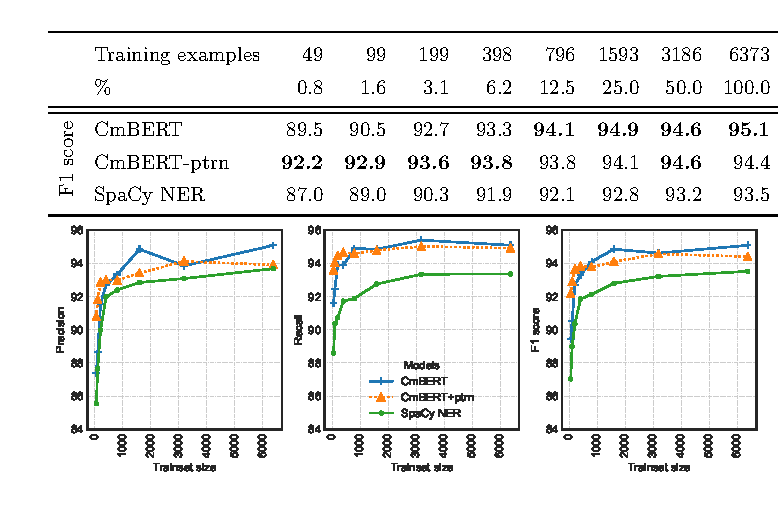
\includegraphics[width=\textwidth]
	       {figs/eval-ner-exp1.pdf}}
	  \caption{\label{fig:f1-vs-trainsize} Metrics measured on the fine-tuned models CmBERT, CmBERT+ptrn and SpaCy NER for 8 training sets of increasing sizes. Precision and recall values are available in the appendix.}
\end{figure}
	                                        


% !TeX root = ../main-paper.tex
\section{Experiment 2: Impact of OCR noise on named entity recognition}
\label{sec:ner-xp2}
Noise introduced by OCR is known to have a negative impact on named entity recognition, because it alters the structure and lexicon of the input texts, moving them away from the language model known to the NER process.
In real-life situations the models used are often trained on texts without such noise, even though the texts to be annotated are extracted with OCR.
This raises the question of the most appropriate strategy to build a NER model tolerant to OCR noise.
In this second experiment we address this question based on our benchmark.


\subsection{Training and evaluation protocol}
Only CmBERT and CmBERT+ptrn are considered since experiment 1 shows that SpaCy NER is systematically outperformed by these two models.

We leverage the labeled sets of entries NER-\emph{reference}, NER-\emph{pero} and NER-\emph{tesseract} created as explained in \cref{sec:dataset}.
Kraken is left aside as it produces poor results that would require removing 500 entries from all datasets to keep the same set of valid entries.

Each dataset is split into a training, a development and a test set following the exact same protocol as described in \cref{sec:ner-xp1-protocol}, except this time we do not need to create smaller training sets.
As the NER sets contain 8341 entries, the producing train sets (resp. development and test) contain 6004 entries - 72\% of the total (resp. 668 - 8\% and 1669 - 20\%).    

CmBERT and CmBERT+ptrn are fine-tuned on the training sets built from NER-\emph{reference} and NER-\emph{pero}.
The training parameters are mostly the same as in \cref{sec:ner-xp1-protocol}, only this time the patience threshold is set to 5 evaluations.
Finally the metrics are measured against the three tests sets.




%\subsubsection{Huggingface CamemBERT}
%\joseph{Copie de \cref{sub:ner-xp1-sysytems-huggingcam}. Je suggère de rédiger la section de l'XP 1 en premier et apporter précision nécessaires ici.}

%Experiments 1 and 2 rely on the implementation of transformers provided by the software library Huggingface (transformers v.4.15.0, datasets v.1.17.0).
%Our baseline CmBERT model is CamemBERT model published on the Hugging Face repository \footnote{\url{https://huggingface.co/Jean-Baptiste/camembert-ner}} and already trained for NER on wikiner-fr.
%Its NER head is a linear model with a Softmax function.
%CmBERT and CmBERT+ptrn are always fine-tuned using the same parameters, with at most 5000 training steps and an early stopping condition set to 3 evaluations in experiment 1 (5 in experiment 2) without improvement of the f1 score. Evaluations are performed every 100 steps.

%\subsection{Protocol}

%We fine-tune CmBERT and CmBERT+ptrn on reference-gold and pero-gold to create two versions of each model: the former trained on manually corrected entries and the latter on OCR entries.
%SpaCy NER is left aside as results from experiment 1 show that it is outperformed by BERT models.
%Performance metrics are computed for each of the four resulting NER models against the test sets created from reference-gold, pero-gold and tesseract-gold.


\subsection{Results and discussion}
The measured F1-score are given in \cref{fig:exp_2_eval_ner}.
Results clearly show that models perform best when both the pre-training and the NER fine-tuning share the same characteristics (here, OCR noise) as the texts to be processed.

In our tests, pre-training the model brings a slight gain in performance ($\approx 0.5\%$).
We did not pre-train or fine-tune with texts extracted with Tesseract.
However, despite a loss of performance, the model pre-trained and fine-tuned on NER-pero still gives the best results.
This is probably due to the fact that the texts produced by Pero-OCR feature characteristics intermediary between human transcriptions and Tesseract.
This OCR tool removes the characters recognised with a low confidence, which is probably a great help to the NER.

\begin{figure}
    \centering
    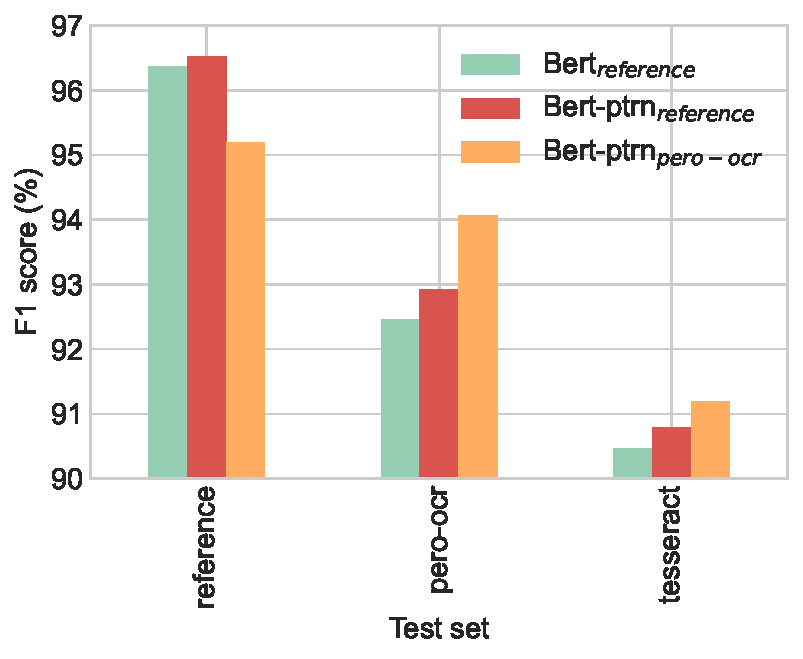
\includegraphics[width=0.75\textwidth]{images/experiment_2_f1_with_noise_graph.pdf}
    \caption{\label{fig:exp_2_eval_ner}F1-scores of NER predictions in presence of OCR noise in the training and testing examples, grouped by test set. The dataset used to train the NER task is noted in indice after the model name (e.g. CmBERT$_{pero}$ means CmBERT fine-tuned on NER-\emph{pero}).}
\end{figure}


% !TeX root = ../main-paper.tex
\section{Conclusion and future works}
We assessed the performance of three modern OCR systems on a set of historical sources of great interest in social history.
Although \peroocr clearly outperforms its competitors, the qualitative analysis of OCR errors shows that its failure cases are not the same as Tesseract.
This calls for leveraging both OCR systems in a complementary way to get the best of the two worlds.
%Moreover, we evaluate two deep-learning-based NER approaches in terms of their sensibility to the amount of training data and to noisy OCR texts.
The evaluation of SpaCy NER and CamemBERT (with and without pre-training) showed that BERT-based NER can benefit from pre-training and fine-tuning on a corpus produced with the same process as the texts to annotate.
%However, the results are not as good as for clean text: it is therefore interesting to investigate how to improve the OCR results or to correct the text in a postprocessing step.
Furthermore, it seems that all three models achieve good performance with relatively few training examples.
With a F1-score of 92\% with only 49 training examples, the pre-trained CamemBERT model is a good choice to serve as a bootstrapping model to quickly produce large training sets and therefore lower the burden of creating a ground truth from scratch.
Besides, as directory entries always have the same structure - at least within a given index - we could take advantage of NER results and some simple rules to identify entries within pages instead of relying on the page layout only, or even interactively generate per-index NER models to take advantage of the low amount of training samples required.
We plan to further explore the robustness of the considered NER models by introducing realistic OCR noise in order to identify possible critical points, in terms of noise level or in terms of entities or structural elements affected.

%Interesting points to discuss:
%\begin{itemize}
%    \item can we train on noisy data? (without manual OCR correction?) => future work? cf Pero OCR training procedure?
%    \item do we need better OCR systems or better post-correction techniques (if NER is reliable enough)?
%    \item Construction of the lexicon and associated cost \nathalie{là je ne comprends pas}
%\end{itemize}
%Ideas for future work:
%\begin{itemize}
%    \item Evaluate this: fine-tune Spacy NER on a few samples to generated a bootstrap dataset, feed it to BERT (cleaned or raw) to create an good model with minimal efforts ? \nathalie{les résultats de la table 2 ne plaident pas vraiment pour ça: même sur les très petits corpus, spacy est tours derrière...}
%    \item Use ML to infer regexes ?
%    \item As directories entries are always structured the same way (in a given list at least): use NER to identify entries within pages to save the burden of having to rely on the page layout ?
%\end{itemize}

\section*{Acknowledgments}
This work is supported by the French National Research Agency (ANR), as part of the SODUCO project, under Grant ANR-18-CE38-0013.
%
The authors want to thank S. Bacciochi and P. Cristofoli for helping to create the reference dataset, 
L. Morice for annotating data,
as well as G. Thomas, P. Abi Saad, R. Lelièvre, D. Mignon, T. Cavaciuti and P. Sadki for contributing to the annotation platform.
%
% Full names
% Stéphane Bacciochi
% Pascal Cristofoli
% Laureencia Morice
% Guillaume Thomas
% Paul Abi Saad
% Raphaël Lelièvre
% Dorian Mignon
% Thibault Cavaciuti
% Pierre Sadki

% ---- Bibliography ----
\bibliographystyle{splncs04}
\bibliography{ref}
\end{document}
